% \section{Lời Cảm Ơn}
\section{Giới thiệu đề tài}

\subsection{Giới thiệu về MIPS}
\indent MIPS - Microprocessor without Interlocked Pipeline Stages - là kiến trúc bộ tập lệnh RISC phát triển
bởi MIPS Technologies. Ban đầu kiến trúc MIPS là 32bit, và sau đó là phiên bản 64 bit. Nhiều sửa đổi
của MIPS, bao gồm MIPS I, MIPS II, MIPS III, MIPS IV, MIPS V, MIPS32 và MIPS64. Phiên bản hiện
tại là MIPS32 và MIPS64.
\subsection{Đề bài 2:}
\textbf{Cộng 2 số thực chuẩn IEEE 754 chính xác đơn.
Viết chương trình thực hiện phép cộng 2 số thực chuẩn IEEE 754 chính xác đơn mà không dùng
các lệnh tính toán số thực của MIPS. Dữ liệu đầu vào đọc từ file lưu trữ dạng nhị phân trên đĩa
FLOAT2.BIN (2 trị x 4 bytes = 8 bytes). 
}\\\\
\textbf{\textit{* Biểu diễn số thực trong máy tính theo chuẩn IEEE 754}}\\\\
Máy tính chỉ có khả năng lưu trữ và xử lý các tín hiệu dưới dạng nhị phân. Do đó, để biểu diễn một số thực trong máy tính, trước tiên chúng ta cần chuyển đổi số đó sang dạng nhị phân. Tuy nhiên, không thể áp dụng cách biểu diễn như đối với số nguyên, mà cần tuân theo một chuẩn riêng biệt – phổ biến nhất là chuẩn \textbf{IEEE 754}.
Chuẩn IEEE 754 quy định hai định dạng chính để biểu diễn số thực.
\begin{itemize}
    \item \textbf{Độ chính xác đơn (single precision)}: sử dụng 32 bit, bao gồm 1 bit dấu, 8 bit cho phần mũ và 23 bit cho phần trị (phần lẻ).
    \item \textbf{Độ chính xác kép (double precision)}: sử dụng 64 bit, bao gồm 1 bit dấu, 11 bit cho phần mũ và 52 bit cho phần trị.
\end{itemize}
\begin{figure}[!h]
    \centering 
    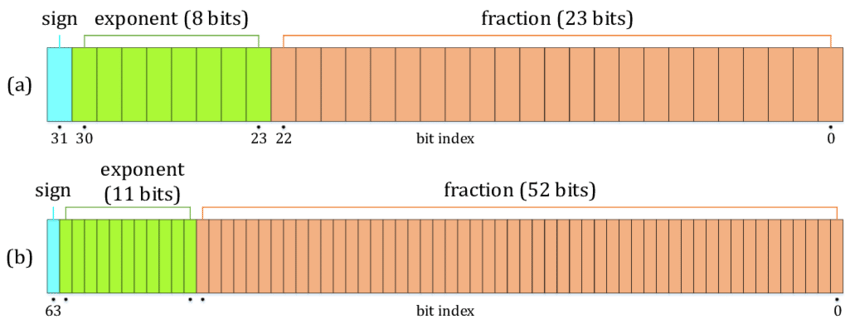
\includegraphics[width=0.8\textwidth]{image/IEEE Standard for Floating-Point Arithmetic (IEEE 754).png}
    \vspace{0.5cm} % khoảng cách sau caption (nếu muốn)
      \caption{ IEEE Standard for Floating-Point Arithmetic (IEEE 754)}
\end{figure}

Trước khi một số thực có thể được lưu trữ theo chuẩn IEEE 754, cần chuyển đổi số đó về \textbf{dạng chuẩn hóa}, tức là biểu diễn sao cho phần nguyên của số không chứa số 0 (ngoại trừ số 0 chính nó).\\

\textbf{\textit{* Thống kê số lượng lệnh R, I, J trong chương trình MIPS}}\\

Trong quá trình phát triển chương trình mô phỏng hợp ngữ MIPS, tổng số lệnh được sử dụng thuộc ba loại R, I và J được thống kê như sau:

\begin{table}[H]
\centering
\begin{tabular}{|c|c|}
\hline
\textbf{Loại lệnh} & \textbf{Số lượng} \\
\hline
R & 20 \\
\hline
I & 36 \\
\hline
J & 4 \\
\hline
\end{tabular}
\caption{Thống kê số lượng lệnh R, I, J sử dụng trong chương trình MIPS}
\end{table}

